\section{Introduction}

Recent advances in large language models (LLMs) have substantially broadened their capabilities, including open-domain dialogue, mathematical reasoning, and program synthesis~\citep{o1, sonnet3_5, Qwen3}. In parallel, tool calling has emerged as a pivotal capability that enables LLMs to interact with external tools such as search engines~\citep{Search-R1, deepresearcher}, calculators~\citep{Schick:2023toolformer, Qin:2024toolllm}, and code interpreters~\citep{PAL, Gou:2024Tora}. By incorporating external tools, LLMs can alleviate fundamental limitations of standalone models, including outdated knowledge and arithmetic errors~\cite{Qin2024:ToolSurvey}. As LLM capabilities continue to improve, tool use increasingly adopts multi-step, multi-turn, feedback-driven interaction loops to solve complex tasks~\cite{gorilla, yao2025taubench}.

\begin{figure}[t]
\centering
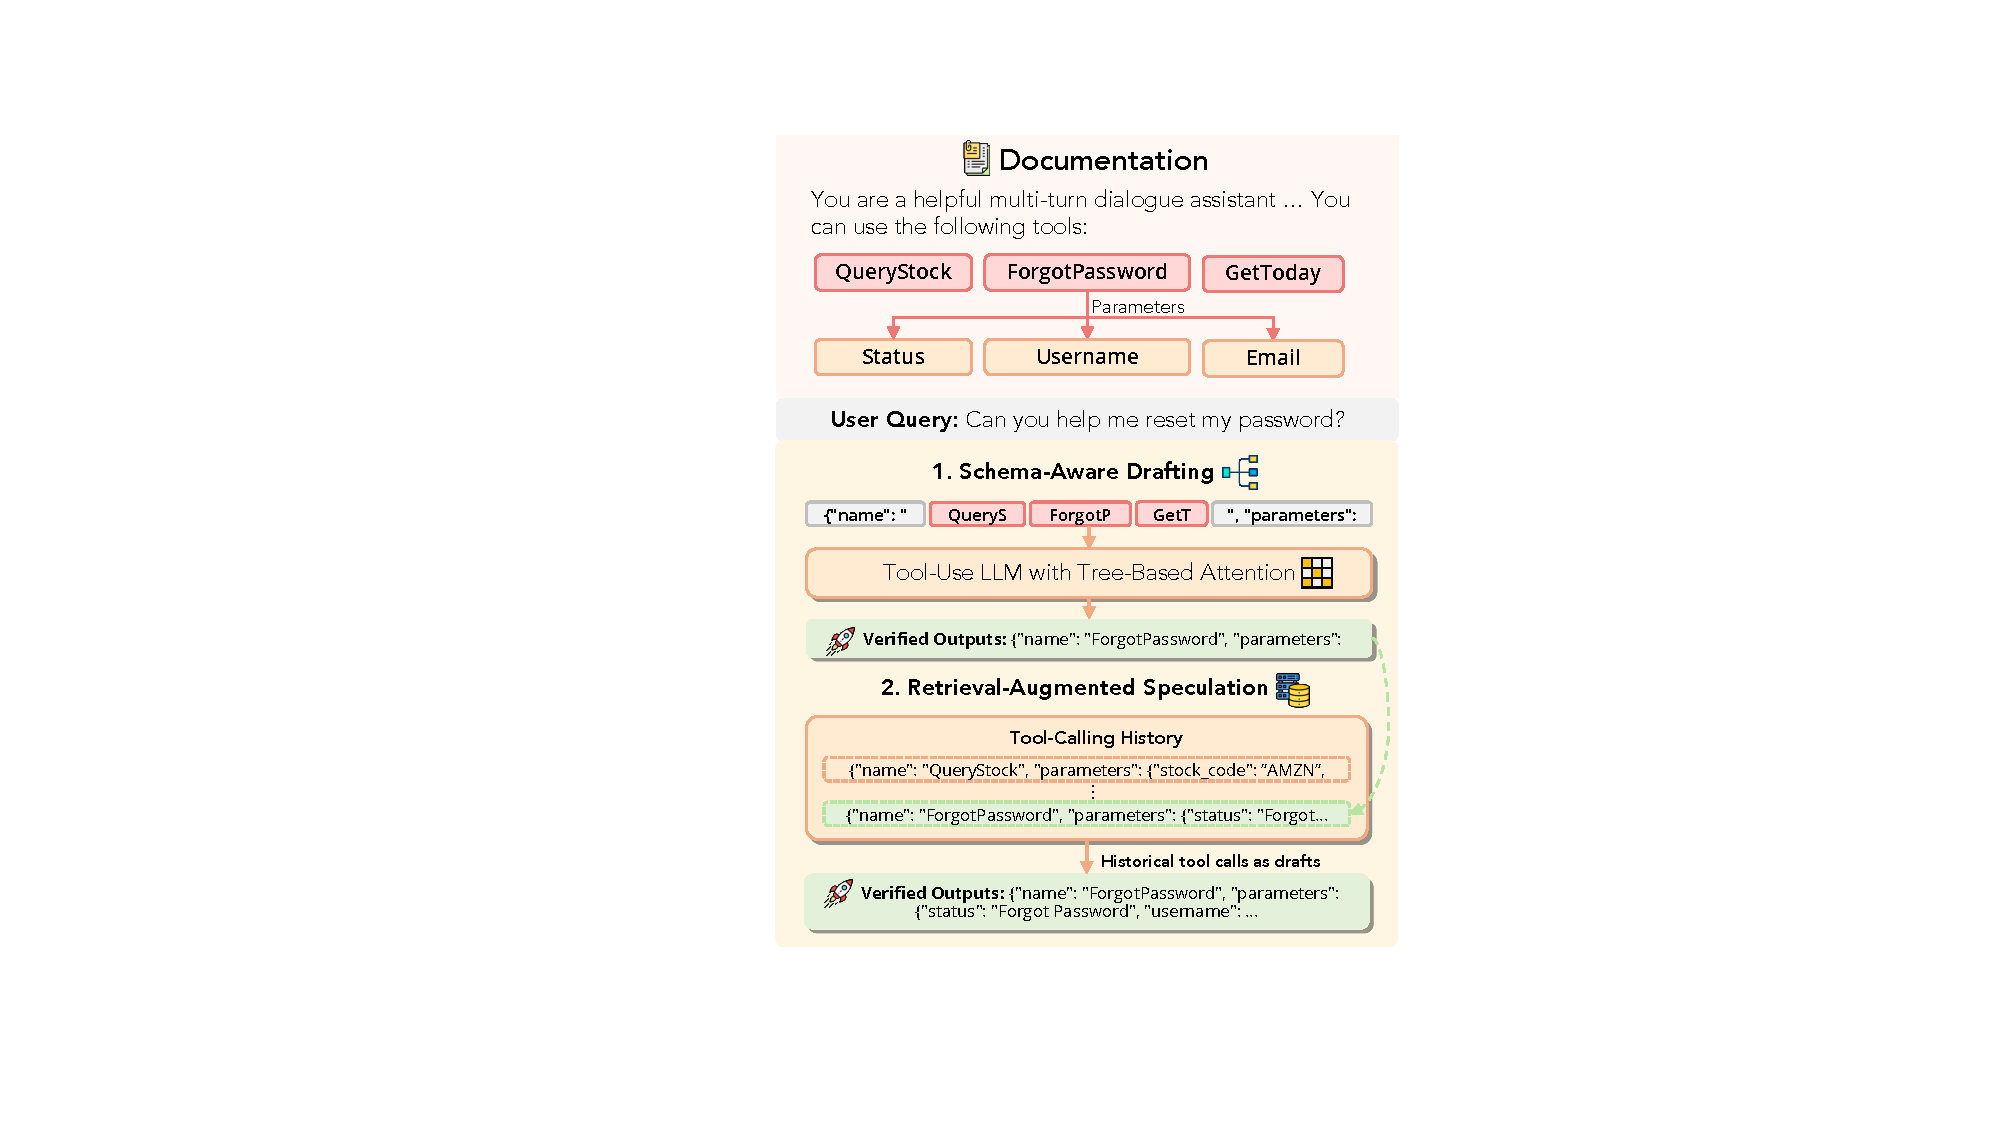
\includegraphics[width=0.95\columnwidth]{fig/intro.pdf}
\caption{Illustration of \method, which accelerates tool-calling generation via two innovations: \textbf{1) schema-aware drafting}, where predefined tool schemas serve as faithful drafts and enable parallel verification of constrained variables (e.g., \colorbox{pink}{tool names}); and \textbf{2) retrieval-augmented speculation}, retrieving and reusing similar historical tool invocations as high-quality drafts.}
\label{fig:intro}
\end{figure}

However, the growing frequency of tool invocations substantially increases inference latency, posing a major challenge for real-time LLM serving. Recent work has proposed several strategies to accelerate tool calling~\cite{LLMCompiler, zhu2025:dividethenaggregate, xu2024conveyor, nichols2025spec}. One line of research models tool-calling trajectories as directed acyclic graphs (DAGs) that capture inter-tool dependencies and then execute independent tools in parallel to reduce overall latency~\cite{LLMCompiler, zhu2025:dividethenaggregate}. Another line improves parallelism by overlapping tool execution with text generation, that is, launching tool calls while the model is still decoding, thereby further accelerating end-to-end tool-calling~\cite{xu2024conveyor, nichols2025spec}. 

Despite these advances in accelerating \textit{tool execution}, this work shifts focus to improving the efficiency of \textit{tool-calling generation}. Our preliminary analysis indicates that generation latency can be a dominant bottleneck: on the widely used benchmark ToolBench~\cite{Qin:2024toolllm}, generating tool calls with Qwen2.5-14B-Instruct accounts for approximately $80\%$ of the end-to-end inference latency and is roughly $4\times$ larger than the time spent executing the tools. Moreover, whereas tool execution time is often relatively stable for a fixed toolset and environment, tool-calling generation latency grows with model size and with the length of the generated tool-call sequence, making it the primary contributor to latency in many tool-using scenarios.

In this work, we present two key observations regarding tool calling: \textbf{1) tool-calling outputs are highly structured.} These outputs are typically expressed in JSON and adhere to strictly constrained schemas. As a result, among the generated tokens, only a small subset corresponds to variable fields, while the rest are schema-determined; \textbf{2) LLMs exhibit recurring tool-call patterns across different requests,} indicating the presence of reusable structural and semantic regularities. Motivated by these insights, we propose \method, a schema-aware and retrieval-augmented speculative decoding (SD) approach for accelerating tool calling. \method leverages the task-specific tool schemas to construct high-quality draft sequences, and employs a finite-state machine to alternate between deterministic schema token filling and speculative generation for variable fields. Furthermore, \method retrieves similar historical tool calls and reuses them as draft candidates, thereby further improving efficiency. Experiments on widely used tool-calling benchmarks, including API-Bank, ToolAlpaca, BFCLv2, and ToolBench, demonstrate that \method achieves up to a $4.2\times$ speedup and outperforms existing SD methods.

We summarize our contributions as follows:
\begin{itemize}
    \item We propose \method, a schema-aware and retrieval-augmented SD approach for accelerating tool-calling generation. It presents a \textit{training-free} solution that can be seamlessly integrated into existing LLM workflows.
    \item Extensive experiments across diverse models and tasks demonstrate that \method consistently achieves a $3.5\times$$\sim$$4.2\times$ speedup, with up to a $71\%$ relative improvement over the previous state-of-the-art SD method.
    \item Further analysis validates the effectiveness of our proposed components and highlights the impact of format adherence on \method’s speedup, indicating its efficiency potential as LLM capabilities continue to advance.
\end{itemize}